% !TeX spellcheck = en_GB
\documentclass[answers]{exam}
% addpoints

\ifprintanswers
	\usepackage{parskip}
	% https://tex.stackexchange.com/a/240769
\fi

\usepackage{tikz}
	\usetikzlibrary{arrows}
\usepackage{circuitikz}

\usepackage{libertine}
% \usepackage[a4paper]{geometry}
\usepackage{amsmath, amsthm, amssymb} 
\usepackage{tabularx}
\usepackage[english]{babel}
\usepackage{enumitem}
\usepackage{gensymb}
\usepackage{bm}
\usepackage{graphicx}
\usepackage{xcolor}
\usepackage{float}
\usepackage{wrapfig}
\usepackage[makeroom]{cancel}
\usepackage{multicol}
\usepackage{vwcol} 	 % Provides variable multicol
\usepackage{commath} % Provides good differentials
\usepackage{siunitx} % Provides good units
\usepackage{nicefrac}
\usepackage{dashrule}
\usepackage[version=4]{mhchem} % for nuclear equations 
% https://tex.stackexchange.com/a/289901

\allowdisplaybreaks

\usepackage[titletoc,title,toc,page]{appendix}
\usepackage{hyperref}
\ifprintanswers
	\hypersetup{
		pdftitle={SJPO Training -- Calculus in Physics Suggested Answers},
		pdfauthor={Sun Yudong, Lor Jun Heng},
		bookmarksnumbered=true,
		bookmarksopen=true,
		bookmarksopenlevel=2,
		pdfstartview=Fit,
		pdfpagemode=UseOutlines,
		colorlinks=true,
		linkcolor=black,
		filecolor=magenta,      
		urlcolor=blue
	}
\else
	\hypersetup{
		pdftitle={SJPO Training -- Calculus in Physics},
		pdfauthor={Lor Jun Heng, Sun Yudong},
		bookmarksnumbered=true,
		bookmarksopen=true,
		bookmarksopenlevel=2,
		pdfstartview=Fit,
		pdfpagemode=UseOutlines,
		colorlinks=true,
		linkcolor=black,
		filecolor=magenta,      
		urlcolor=blue
	}
\fi

\newcommand{\uvec}[1]{\boldsymbol{\hat{\textbf{#1}}}}
\def\doubleunderline#1{\underline{\underline{#1}}}

\renewcommand{\ttdefault}{cmtt}

\newenvironment{multicolFigure}
{\par\medskip\noindent\minipage{\linewidth}}
{\endminipage\par\medskip}

\ifprintanswers
	\title{SJPO Training\\ Calculus in Physics\\ {\Large --- Suggested Answers ---}}
	\author{Sun Yudong, Lor Jun Heng}
	\date{Feb 21, 2019}
\else
	\title{SJPO Training\\ Calculus in Physics}
	\author{Lor Jun Heng, Sun Yudong}
	\date{Feb 2, 2019}
\fi

\begin{document}
\maketitle

\ifprintanswers
	This worksheet was meant to be notes/questions to complement the lesson. The ``answers" provided are just so you can kind of grasp what is going on.
\fi

\section*{Differentiation and Differential Equations}
\begin{questions}

	\question{A nuclear fission reaction occurs when a neutron collides and joins with an atomic nucleus, causing the new nucleus to be energetically unstable. Neutrons, smaller daughter nuclei and energy are released as products of the nuclear reaction. Can a chain reaction be sustained if there are many more daughter nuclei than neutrons? What will happen to the reaction if there are fewer daughter nuclei than neutrons and some some of the neutrons escape the reacting system?
		\begin{solution}
			\setlength{\parskip}{1.2\bigskipamount plus \smallskipamount minus \smallskipamount}
			Okay, the point is not actually about getting the answers to the questions themselves, but to just get you used to the idea of differential equation -- situations where you have different orders of differentials in the same equation, and to introduce to you the concept of separation of variables. Now to the question itself:

			For the first part, it is to provide you with a qualitative understanding of how nuclear fission works -- if there is a greater number of neutrons, there will be more and higher frequency of collisions and thus a higher rate of reaction. 


			Let's say that the following fictional reactions takes place:
			\begin{equation}
				\ce{^238X -> ^236X +  2^1n + \gamma } 
			\end{equation}
			We can deduce a rate equation from this in the form of:
			\begin{equation}
				\text{Rate} = k\left[\ce{^238X}\right]
			\end{equation}
			where $[\ce{Y}]$ represents the concentration of $\ce{Y}$ and $k$ is the rate constant.

			% For most situations though, the number of particles of $\ce{^238X}$ is much much more than the number of neutrons in the reaction mixture. Thus, whenever a bit of $\ce{^238X}$ is reacted away, the concentration $\left[\ce{^238X}\right]$ does not change significantly. Thus, we can approximate it to be constant to give the following:
			% \begin{equation}
			% 	\text{Rate} = k\left[\ce{^238X}\right]\left[\ce{^1n}\right] = k'\left[\ce{^1n}\right]
			% \end{equation}

			Changing everything from concentration to the actual number of particles, rate can be expressed as $\dod{N}{t}$ where $N$ is number of $\ce{^238X}$ to obtain:
			\begin{equation}
				\dod{N}{t} = kN = -\lambda N
			\end{equation}
			which is a first order differential equation. We choose to add a negative sign since we know that $N$ is decreasing over time. 

			We can solve for $N\!\left(t\right)$ by first separating the variables, and then integrating both sides:
			\begin{align}
				\frac{1}{N} \dif{N} &= -\lambda \dif{t} \notag \\
				\int_{N_0}^{N\!\left(t\right)} \frac{1}{N} \dif{N} &= \int_0^t -\lambda  \dif{t} \notag \\
				\left[\ln{N}\right]_{N_0}^{N\!\left(t\right)} &= \left[-\lambda t\right]_0^t \notag \\
				\ln{N\!\left(t\right)} - \ln{N_0} &= -\lambda t \notag \\
				\ln{\frac{N\!\left(t\right)}{N_0}} &= -\lambda t \notag \\
				N\!\left(t\right) &= N_0e^{-\lambda t} \label{eqn:expDecay}
			\end{align}
			Equation \eqref{eqn:expDecay} is the classic equation that describes Exponential Decay.

			The half life of the sample (the time taken for the number of $\ce{^238X}$ to decrease by half) is then given by:
			\begin{equation}
				t_{\nicefrac{1}{2}} = \frac{\ln 2}{\lambda}
			\end{equation}
			Do note that the manipulation we used to obtain \eqref{eqn:expDecay} exists purely in Physics and not Math.
		\end{solution}
	}

	\question{Imagine a rocket at rest in space with no forces exerted on it. However, as soon as its engine is started (clock set to 0), the rocket is expelling gas mass at a constant mass flow rate $M \left(\si{\kilo\gram\per\second}\right)$ and at exhaust velocity relative to the rocket $v_e \left(\si{\meter\per\second}\right)$ Find an equation which relates the velocity of the rocket with mass of the rocket?
		\begin{solution}
			This question is to get you to appreciate the idea that in Physics, it is often the case that you \textit{\textbf{have to}} use calculus in order to obtain an answer. This results often from how many physical properties change as a result of something else changes. 

			In this case, if you tried to apply the Conservation of Linear Momentum directly to the entire rocket and fuel, it isn't that easy to solve as each $\dif{m}$ of mass ejected from the rocket will be going at a different velocity from the previous one due to the increasing velocity of the rocket. Writing the following, for example, will be wrong:
			\begin{equation}
				\Delta P = 0 = \left[\left(M_r - \dif{m}\right)v_r\right] + \left[v_e\dif{m}\right] ~~~~ \text{\textcolor{red}{wrong!}}
			\end{equation}
			If we want to write the above, we need to consider that the velocity of the ejected fuel $V_e = v_e - v_r$ is actually a function of time $t$ and is not the constant $v_e$. 

			So let us consider the following system in one moment in time from the point of view of a stationary observer:
			\begin{center}
				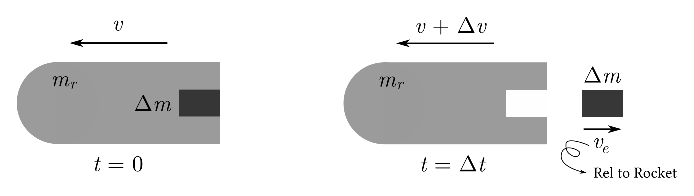
\includegraphics[width=0.8\textwidth]{rocket_system.eps}
			\end{center}
			where $m_r$ is the mass of the rocket and any unburnt propellant.

			At time $t = 0$, the momentum $P_i$ can be written as:
			\begin{equation}
				P_i = \left(m_r + \Delta m\right)v
			\end{equation}
			At time $t = \Delta t$, the momentum $P_{f}$ can be written as:
			\begin{equation}
				P_{f} = \left(v + \Delta v\right)m_r + V_e \Delta m
			\end{equation}
			where $V_e = v - v_e$.

			By Newton's 2\textsuperscript{nd} Law, we have:
			\begin{align*}
				\sum F_\text{internal} &= \lim_{\Delta t \to 0} \frac{P_f - P_i}{\Delta t} \\
				& = \lim_{\Delta t \to 0}\frac{\left[\left(v + \Delta v\right)m_r + V_e \Delta m\right] - \left[\left(m_r + \Delta m\right)v\right]}{\Delta t} \\
				& = \lim_{\Delta t \to 0}\frac{\cancel{m_rv} + m_r\Delta v + V_e \Delta m - \cancel{m_rv} - v\Delta m}{\Delta t} \\
				& = \lim_{\Delta t \to 0}\frac{m_r\Delta v + \left(\cancel{v} - v_e\right) \Delta m - \cancel{v\Delta m}}{\Delta t} \\
				& = \lim_{\Delta t \to 0}\frac{m_r\Delta v - v_e\Delta m}{\Delta t} 
			\end{align*}
			The rocket ejects a positive mass that results in a $\dod{m}{t} < 0$, thus we can take $\dif{m} = -\Delta m$:
			\begin{equation}
				\sum F_\text{internal} = m_r \dod{v}{t} + v_e \dod{m}{t}
			\end{equation}
			Since there are no external forces on the system:
			\begin{equation}
				m_r \dod{v}{t} = -v_e \dod{m}{t}
			\end{equation}
			Separating the variables and integrating:
			\begin{align*}
				\int_0^t \dod{v}{t} \dif t &= - v_e \int_0^t \frac{1}{m} \dod{m}{t} \dif{t} \\ 
				\left[v\right]^{v\left(t\right)}_{v_0} &= -v_e\left[\ln{m}\right]^{m\left(t\right)}_{m_0} \\
				v - v_0 &= -v_e\left[\ln m - \ln m_0\right] \\
				\Delta v &= v_e\ln{\frac{m_0}{m}}
			\end{align*}
			which yields the Tsiolkovsky rocket equation.

			As you can see, in a case like this, calculus must be used in order to easily and properly consider the problem.

			This however does not consider any relativistic effects. The modification to consider these effects are left as an exercise for the reader. 
		\end{solution}
	}
\end{questions}
\ifprintanswers
	\pagebreak
\fi
\section*{Integration}
\begin{questions}

	\question{For a sphere of density $\rho$ tho and radius $R$, integrate the infinitesimal mass elements to find the mass of the sphere when:
		\begin{parts}
			\part $\rho$ is constant
			\part $\rho$ is proportional to $R$
			\part $\rho$ is inversely proportional to $R$
		\end{parts}

		\begin{solution}
			\par 
			\begin{tabularx}{\textwidth}{@{} X X X @{}}
				(a) $\rho$ is constant & (b) $\rho$ is proportional to $R$ & (c) $\rho$ is inversely proportional to $R$ \\
				{\begin{align*}
 					M &= \int^V_0 \dif{V} \cdot \rho \\
 					&= \int^R_0 4\pi r^2 \rho \dif{r} \\
 					&= 4\pi\rho \int^R_0 r^2 \dif{r} \\
 					&= \frac{4}{3}\pi\rho R^3 %
 				\end{align*}} & %
				{\begin{align*}
					M &= \int^V_0 \dif{V} \cdot \rho \\
					&= \int^R_0 4\pi r^2 \left(kr\right) \dif{r} \\
					&= 4\pi k \int^R_0 r^3 \dif{r} \\
					&= \pi k R^4 %
				\end{align*}} & %
				{\begin{align*}
					M &= \int^V_0 \dif{V} \cdot \rho \\
					&= \int^R_0 4\pi r^2 \left(k \cdot \frac{1}{r}\right) \dif{r} \\
					&= 4\pi k \int^R_0 r \dif{r} \\
					&= 2\pi k R^2 %
				\end{align*}}
			\end{tabularx}
		\end{solution}
	}

	\question{A block of mass $M$ sliding down slope of angle $\theta$ and coefficient of friction $\mu_k$ is proportional to time. Find the equation describing the velocity of the block as a function of time?

	\textit{Some variants}: what's the behaviour of the block for different constant coefficient of friction? What if the coefficient of friction is proportional to the slant distance?
		
		\begin{solution} \par
		\vspace{-2em}
			\begin{tabularx}{\textwidth}{@{} X p{5cm} @{}}
				{\begin{align*}
 					\sum F_\text{net} &= M\!g\sin\theta - \mu_k N \\
 					&= M\!g\sin\theta - \left(kt\right)\left(M\!g\cos\theta\right) \\
 					\implies a = \dod{v}{t} &= g\sin\theta - gkt\cos\theta \\
 					\int^t_0 \dod{v}{t} \dif{t} &= \int^t_0 g\sin\theta - gkt\cos\theta \dif{t} \\
 					&= \left[gt\sin\theta - gk\cos\theta \cdot \frac{t^2}{2}\right]^t_0 \\
 					v &= v_0 + gt \left[\sin\theta - \frac{1}{2}k\cos\theta t\right] 
 				\end{align*}} & 
				{\begin{center}
					\centering
					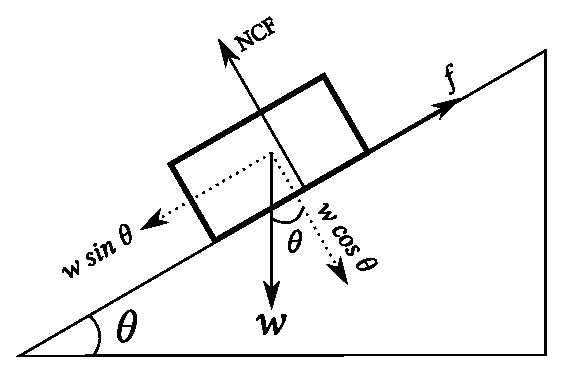
\includegraphics[width=4.5cm]{slope.eps}
				\end{center}}
			\end{tabularx}
			The variants are left as an exercise for the reader. General descriptions:
			\begin{enumerate}[label=(\roman*)]
				\item The block will experience a constant acceleration if the coefficient of friction $\mu_k$ is constant. % $v = v_0 + gt \left(\sin\theta - \mu_k \cos\theta\right)$ \par
				\item The block decelerates at an increasing rate (the decreasing part of a positive sine curve).
			\end{enumerate}
		\end{solution}
	}

	\question{Calculate the moments of inertia $I$ using $\dif{I} = r^2 \dif{m}$. The mass is evenly distributed in the objects below:
		\begin{parts}
			\part A stick of mass $M$ and length $L$ at the centre.
			\part The same but at one end.
			\part A flat disc at the centre.
		\end{parts}

		\begin{solution}
			\begin{multicols}{2}
				\begin{enumerate}[label=(\alph*)]
					\item \textcolor{white}{.}
					\vspace{-2.8em}
						\begin{align*}
							I &= 2\int^{\nicefrac{M}{2}}_0 r^2 \dif{m} \\
							&= 2\int^{\nicefrac{L}{2}}_0 r^2 \left(\frac{M}{L}\right) \dif{r} \\
							&= \frac{2M}{L} \left[\frac{r^3}{3}\right]^{\nicefrac{L}{2}}_0 \\
							&= \frac{2M}{L} \cdot \frac{L^3}{24} \\
							&= \frac{1}{12}M\!L^2
						\end{align*}
					\item \textcolor{white}{.}
					\vspace{-3.2em}
						\begin{align*}
							I &= \int^M_0 r^2 dm \\
							&= \int^L_0 r^2 \left(\frac{M}{L}\right) \dif{r} \\
							&= \frac{M}{L} \left[\frac{r^3}{3}\right]^L_0 \\
							&= \frac{M}{L} \cdot \frac{L^3}{3} \\
							&= \frac{1}{3}M\!L^2
						\end{align*}
				\end{enumerate}
			\end{multicols}
			(c)
			\vspace{-2em}
			\begin{align*}
				V = \pi R^2 h &\implies \dif{V} = 2\pi hR \dif{r} \\
				\implies I_z &= \rho \int^V_0 r^2 \dif{V} \\
				&= \frac{M}{V} \int^R_0 r^2 \left(2\pi h r\right) \dif{r} \\
				&= \frac{M}{\cancel{\pi R^2h}} \left(\cancel{2\pi h}\right) \cdot \frac{R^{\cancelto{2}{4}}}{\cancelto{2}{4}} \\
				&= \frac{1}{2}M\!R^2
			\end{align*}
		\end{solution}
	}
	\ifprintanswers
		\pagebreak
	\fi
	\question{A metal sphere of mass $M$ is falling through a viscous fluid and it experiences a drag force, $b$, which is proportional to its velocity. Find the equation which describes the motion of the sphere.

		\begin{solution}
		\par
			\vspace{-3.4em}
			\begin{align*}
				F_\text{net} &= mg - kv \\
				a &= g - \frac{k}{m} v\\
				\frac{1}{g-\frac{k}{m} v} \cdot \dod{v}{t} &= 1 \\
				\int^t_0 \frac{1}{g-\frac{k}{m} v} \cdot \dod{v}{t} \dif{t} &= \int^t_0 1 \dif{t} \\
				-\frac{m}{k}\left[\ln{\left| g - \frac{k}{m}v \right|}\right]^v_0 &= t \\
				-\frac{m}{k}\left[\ln{\left| g - \frac{k}{m}v \right|} - \ln{g}\right] &= t \\ 
				\ln{\left| 1 - \frac{k}{mg}v \right|} &= -\frac{kt}{m} \\
				\left| 1 - \frac{k}{mg}v \right| &= e^{-kt/m} \\
				v &= \frac{mg}{k}\left(1-Ae^{-kt/m}\right)
			\end{align*}
			where $A = \pm 1$ depending on the initial conditions.
		\end{solution}
	}
\end{questions}

\ifprintanswers
	\vspace{5em}

	As you can see, a lot physics questions involve calculus and it can get quite difficult to analyse questions if you do not have the necessary mathematical tools to aid you. In most of these questions, you realize that you first find some form of differential equation to describe the physics, and then solve this differential equation to obtain the property that you would like to describe. 
\fi

\end{document}